%%%%%%%%%%%%%%%%%%%%%%%%%%%%%%%%%%%%%%%%%
% University Assignment Title Page 
% LaTeX Template
% Version 1.0 (27/12/12)
%
% This template has been downloaded from:
% http://www.LaTeXTemplates.com
%
% Original author:
% WikiBooks (http://en.wikibooks.org/wiki/LaTeX/Title_Creation)
%
% License:
% CC BY-NC-SA 3.0 (http://creativecommons.org/licenses/by-nc-sa/3.0/)
% 
% Instructions for using this template:
% This title page is capable of being compiled as is. This is not useful for 
% including it in another document. To do this, you have two options: 
%
% 1) Copy/paste everything between \begin{document} and \end{document} 
% starting at \begin{titlepage} and paste this into another LaTeX file where you 
% want your title page.
% OR
% 2) Remove everything outside the \begin{titlepage} and \end{titlepage} and 
% move this file to the same directory as the LaTeX file you wish to add it to. 
% Then add \input{./title_page_1.tex} to your LaTeX file where you want your
% title page.
%
%%%%%%%%%%%%%%%%%%%%%%%%%%%%%%%%%%%%%%%%%
%\title{Title page with logo}
%----------------------------------------------------------------------------------------
%	PACKAGES AND OTHER DOCUMENT CONFIGURATIONS
%----------------------------------------------------------------------------------------

\documentclass[12pt]{article}
\usepackage[english]{babel}
\usepackage[utf8x]{inputenc}
\usepackage{amsmath}
\usepackage{graphicx}
\usepackage[colorinlistoftodos]{todonotes}

\begin{document}
\begin{titlepage}

\newcommand{\HRule}{\rule{\linewidth}{0.5mm}} % Defines a new command for the horizontal lines, change thickness here

\center % Center everything on the page
 
%----------------------------------------------------------------------------------------
%	HEADING SECTIONS
%----------------------------------------------------------------------------------------

\textsc{\LARGE National School of Geographic Sciences}\\[0.2cm] % Name of your university/college

%----------------------------------------------------------------------------------------
%	LOGO SECTION
%----------------------------------------------------------------------------------------


\includegraphics[scale=0.4]{../images/logo.png}\\[0.2cm] % Include a department/university logo - this will require the graphicx package
 
%----------------------------------------------------------------------------------------

\textsc{\Large Geomatics and Information Systems Technology}\\[0.5cm] % Major heading such as course name
%\textsc{\large Minor Heading}\\[0.5cm] % Minor heading such as course title

%----------------------------------------------------------------------------------------
%	TITLE SECTION
%----------------------------------------------------------------------------------------

\HRule \\[0.4cm]
{ \huge \bfseries Architectural Patterns}\\[0.4cm] % Title of your document
{ \bfseries ex MapReduce}\\[0.2cm] % Title of your document
\HRule \\[1.5cm]
 
%----------------------------------------------------------------------------------------
%	AUTHOR SECTION
%----------------------------------------------------------------------------------------

\begin{minipage}{0.4\textwidth}
\begin{flushleft} \large
\emph{Author:}\\
Mohamed Amjad \textsc{LASRI} % Your name
\end{flushleft}
\end{minipage}
~
\begin{minipage}{0.4\textwidth}
\begin{flushright} \large
\emph{Supervisor:} \\
Emmanuel \textsc{Bardiere} % Supervisor's Name
\end{flushright}
\end{minipage}\\[2cm]

% If you don't want a supervisor, uncomment the two lines below and remove the section above
%\Large \emph{Author:}\\
%John \textsc{Smith}\\[3cm] % Your name

%----------------------------------------------------------------------------------------
%	DATE SECTION
%----------------------------------------------------------------------------------------

{\large \today}\\[1cm] % Date, change the \today to a set date if you want to be precise


\vfill % Fill the rest of the page with whitespace

\end{titlepage}


\begin{abstract}
Architectural patterns provide reusable solutions for common architectural problems. Patterns usually don't contains code that you can cut and past; instead, they contain architectural and design information that you build into your solution.
Nowadays we define architectural patterns sub-domains adapted, more or less, to each type of situations. In this documentary research project we presente what architectural patterns are, How are they integrated into an information system project?  We also provide 

\end{abstract}

\renewcommand{\abstractname}{Acknowledgements}
\begin{abstract}
 Thanks God, thanks Mum!
\end{abstract}

\renewcommand{\abstractname}{License}
\begin{abstract}
    Copyright (C)  2014  Mohamed Amjad LASRI.
    Permission is granted to copy, distribute and/or modify this document
    under the terms of the GNU Free Documentation License, Version 1.3
    or any later version published by the Free Software Foundation;
    with no Invariant Sections, no Front-Cover Texts, and no Back-Cover Texts.
    A copy of the license is included in the section entitled "GNU
    Free Documentation License".
\end{abstract}


\section{Introduction}

Architectural patterns are commonly recognised as efficient solutions to a reccuring problem in the software architecture field. This type of patterns is generally implemented to solve some problems related to hardware performance, business risks, big data analysis, servers high availability ...and others.
nevertheless, "Architectural patterns" is a confusing expression, the reader must distinguish between this expression and "software architecture styles". For example, SOA is a software architecture style, but ESB -which is an architectural pattern- is a manner to implemente a SOA.
In the schema diagram bellow we presente some software architecture style and the related architectural patterns.
The reader must also distinguish between two others confusing concepts: design patterns and architectural patterns:
 Design patterns are usually associated with code level commonalities. It provides various schemes for refining and building smaller subsystems. It is usually influenced by programming language. Some patterns pale into insignificance due to language paradigms. Design patterns are medium-scale tactics that flesh out some of the structure and behavior of entities and their relationships.

While architectural patterns are seen as commonality at higher level than design patterns. Architectural patterns are high-level strategies that concerns large-scale components, the global properties and mechanisms of a system.

\section{Architectural Patterns}
\label{sec:ArchitecturalPatterns}

In this section we list some basic architectural styles and the patterns that help you design them. There may be more than one pattern for each style. Both MVC and PAC, for example, are in the interactive system style.

\subsection{From Mud to Structure}
From Mud to Structure is the root and entry point to our pattern language. Its featured patterns help to transform the mud of requirements and constraints we usually start with into a coarse-grained software structure with clearly separated, tangible parts that make up the system being developed, and address several key concerns of sustainable software architectures: operational aspects such as performance and availability, as well as developmental qualities like extensibility and maintainability.

\subsubsection{Layered Architecture}
an example of a "From Mud to Structure" pattern is the layered architecture. This architectural pattern have been since the beginning of digital computers — or at least since the early 1960s. Modern hardware technology and languages accentuate the usefulness of layered architectures.
The International Standards Organization (ISO) Open Systems Interconnection (OSI) seven-layer model (see the Figure bellow) facilitates communication between computers. The model consists of two separate but parallel stacks of layers; each layer provides a higher level of functionality than the layer below it.
Within the two stacks, the layer N in one stack is a peer of the layer N in the other stack. Logically, communication is between the peer layers in the two stacks; actually, only the bottommost layer directly communicates between the two stacks.

% Include the OSI figure
\begin{figure}
\centering
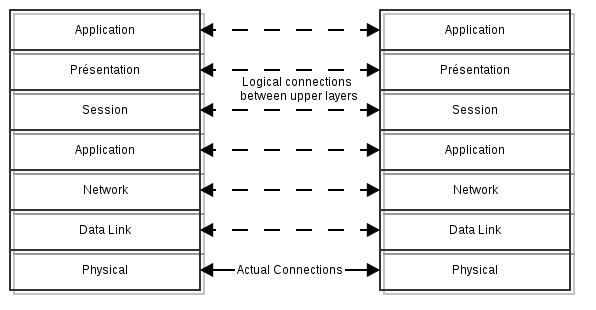
\includegraphics[width=1\textwidth]{../images/osi_model.png}
\caption{\label{fig:frog} the OSI architectural pattern}
\end{figure}

Layers can be different sizes, hosting different numbers of protocols. Over time, in fact, the communications-stack diagram has evolved into many variations. Some layers have many alternatives — such as SIP, FTP, Telnet, and HTTP in layer 7 (the Application layer) — and other layers have few alternatives.
Something that’s true of layered architectures in general is true of the OSI model as well: Changes to a layer affect only that one layer. In other words, the communication protocol chosen at a lower layer doesn’t affect the higher- level functionality provided at its higher level. You’re free to pick and choose the protocols to use in each layer — just keep in mind that for peers to talk to each other, the peer layers in the two stacks must use the same protocol.

\subsection{Distributed systems}
A distributed system consists of a collection of autonomous nodes (computers or servers), connected through a network and distribution middleware, which enables computers to coordinate their activities and to share the resources of the system, so that users perceive the system as a single, integrated computing facility.
The most known architectural patterns that implemente the distributed systems architecture:
\begin{itemize}
\item 2-tiers (client-server), 3-tiers, n-tiers,
\item Peer-to-Peer,
\item Broker,
\item Serivce Oriented,
\end{itemize}

\subsection{Sections}

Use section and subsection commands to organize your document. \LaTeX{} handles all the formatting and numbering automatically. Use ref and label commands for cross-references.

\subsection{Comments}

Comments can be added to the margins of the document using the \todo{Here's a comment in the margin!} todo command, as shown in the example on the right. You can also add inline comments too:

\todo[inline, color=green!40]{This is an inline comment.}

\subsection{Tables and Figures}

Use the table and tabular commands for basic tables --- see Table~\ref{tab:widgets}, for example. You can upload a figure (JPEG, PNG or PDF) using the files menu. To include it in your document, use the includegraphics command as in the code for Figure~\ref{fig:frog} below.

% Commands to include a figure:
\begin{figure}
\centering

\includegraphics[width=0.5\textwidth]{../images/logo.png}
\caption{\label{fig:frog}This is a figure caption.}
\end{figure}

\begin{table}
\centering
\begin{tabular}{l|r}
Item & Quantity \\\hline
Widgets & 42 \\
Gadgets & 13
\end{tabular}
\caption{\label{tab:widgets}An example table.}
\end{table}

\subsection{Mathematics}

\LaTeX{} is great at typesetting mathematics. Let $X_1, X_2, \ldots, X_n$ be a sequence of independent and identically distributed random variables with $\text{E}[X_i] = \mu$ and $\text{Var}[X_i] = \sigma^2 < \infty$, and let
$$S_n = \frac{X_1 + X_2 + \cdots + X_n}{n}
      = \frac{1}{n}\sum_{i}^{n} X_i$$
denote their mean. Then as $n$ approaches infinity, the random variables $\sqrt{n}(S_n - \mu)$ converge in distribution to a normal $\mathcal{N}(0, \sigma^2)$.

\subsection{Lists}

You can make lists with automatic numbering \dots

\begin{enumerate}
\item Like this,
\item and like this.
\end{enumerate}
\dots or bullet points \dots
\begin{itemize}
\item Like this,
\item and like this.
\end{itemize}

We hope you find write\LaTeX\ useful, and please let us know if you have any feedback using the help menu above.

\end{document}
